% !TeX root = surprises.tex

\selectlanguage{hebrew}


\chapter{אפשר להסתפק במחוגה}\label{c.compass}

%%%%%%%%%%%%%%%%%%%%%%%%%%%%%%%%%%%%%%%%%%%%%%%%%%%%%%%%%%%%%%%

בשנת
$1797$
הוכיח לורנצו מסקרוני 
\L{Lorenzo Mascheroni}
שכל בנייה גיאומטרית באמצעות סרגל ומחוגה ניתנת לבנייה במחוגה בלבד. במאה ה-20 התגלה שהמשפט הוכח בשנת
$1672$
על ידי גיאורג מור
\L{(Georg Mohr)}.
המשפט נקרא היום משפט מור-מסקרוני
לאחר שנסביר בסעיף%
~\ref{s.compass-what}
מה המשמעות של בניות ללא מחוגה, נביא את ההוכחה בשלבים, תחילה עם ארבע בניות עזר: שיקוף של נקודה (סעיף%
~\ref{s.reflection}),
בניית מעגל עם רדיוס נתון (סעיף%
~\ref{s.circle}),
חיבור וחיסור קטעים (סעיף%
~\ref{s.add-subtract})
ובניית קטע כיחס בין קטעים אחרים (סעיף%
~\ref{s.three}).
סעיף%
~\ref{s.two-lines}
מראה איך למצוא את החיתוך בין שני ישרים וסעיף%
~\ref{s.line-circle}
מראה איך למצוא את החיתוך בין ישר ומעגל.

%%%%%%%%%%%%%%%%%%%%%%%%%%%%%%%%%%%%%%%%%%%%%%%%%%%%%%%%%%%%%%%

\section{מהי בנייה במחוגה בלבד?}\label{s.compass-what}

איור%
~\ref{f.compass-equi}
מראה את הבנייה הרגילה של משולש שווה צלעות בסרגל ומחוגה. איך אפשר לבנות משולש ללא הקטעים
$\overline{AB},\overline{AC},\overline{BC}$?
למעשה, אין כל צורך
\textbf{לראות}
את הקטעים. קטע מוגדר על ידי שתי נקודות, ומספיק לבנות את הנקודות 
$A,B,C$
 כדי לקבל בנייה שקולה לבנייה בסרגל 
(איור%
~\ref{f.compass-equi-only}).
באיורים נצייר בכל זאת קווים, אולם הקווים משמשים אך ורק להבנת הבנייה ולהוכחת נכונותה. חשוב להשתכנע שהבנייה עצמה משתמשת רק במחוגה.

\begin{figure}[bt]
\begin{center}
\begin{subfigure}{.4\textwidth}
\begin{tikzpicture}[scale=0.6]
\coordinate (A) at (0,0);
\coordinate (B) at (4,0);
\path (A) node[below left] {$A$} -- (B) node[below right] {$B$};
\fill (A) circle[radius=2pt];
\fill (B) circle[radius=2pt];
\draw[name path=larc] (A) ++(-10:4cm) arc (-10:80:4cm);
\draw[name path=rarc] (B) ++(-170:4cm) arc (-170:-260:4cm);
\path [name intersections={of=larc and rarc,by={t}}];
\fill (t) node[above right,xshift=-2pt,yshift=3pt] {$C$} circle[radius=2pt];
\end{tikzpicture}
\caption{בניית משולש שווה צלעות בסרגל ומחוגה}\label{f.compass-equi}
\end{subfigure}
\hspace{3em}
\begin{subfigure}{.4\textwidth}
\begin{tikzpicture}
\coordinate (A) at (0,0);
\coordinate (B) at (4,0);
\draw (A) node[below left] {$A$} -- (B) node[below right] {$B$};
\fill (A) circle[radius=2pt];
\fill (B) circle[radius=2pt];
\draw[name path=larc] (A) ++(-10:4cm) arc (-10:80:4cm);
\draw[name path=rarc] (B) ++(-170:4cm) arc (-170:-260:4cm);
\path [name intersections={of=larc and rarc,by={t}}];
\fill (t) node[above right,xshift=-2pt,yshift=3pt] {$C$} circle[radius=2pt];
\draw (A) -- (t);
\draw (B) -- (t);
\end{tikzpicture}
\caption{בניית משולש שווה צלעות במחוגה בלבד}\label{f.compass-equi-only}
\end{subfigure}
\end{center}
\end{figure}
כל צעד בבנייה באמצעות סרגל ומחוגה הוא אחת משלוש הפעולות הבאות:
\begin{itemize}
\item
מציאת נקודת החיתוך של שני ישרים.
\item
מציאת נקודות החיתוך של ישר ומעגל.
\item
מציאת נקודות החיתוך של שני מעגלים.
\end{itemize}
ניתן לבצע את הפעולה השלישית במחוגה בלבד. עלינו להראות שעבור שתי הפעולות הראשונות ניתן למצוא בנייה שקולה שמשתמשת במחוגה בלבד.

נשתמש בסימונים:
\begin{itemize}
\item $c(O,A)$: 
מעגל שמרכזו
$O$
ועובר דרך הנקודה
$A$.
\item $c(O,r)$:
מעגל שמרכזו
$O$
ורדיוסו
$r$.
\item $c(O,\overline{AB})$:
מעגל שמרכזו
$O$
ורדיוס באורך הקטע
$\overline{AB}$.
\end{itemize}

%%%%%%%%%%%%%%%%%%%%%%%%%%%%%%%%%%%%%%%%%%%%%%%%%%%%%%%%%%%%%%%

\section{שיקוף נקודה}\label{s.reflection}

\begin{definition}
הנקודה
$C'$
היא
\textbf{%
שיקוף%
}
של הנקודה
$C$
ביחס לקטע 
$\overline{AB}$,
אם 
$\overline{AB}$
(או הישר המכיל אותו) הוא האנך האמצעי של
$\overline{CC'}$.
\end{definition}
\begin{theorem}\label{thm.reflection}
נתון קטע 
$\overline{AB}$
ונקודה 
$C$
שלא נמצאת על
$\overline{AB}$,
ניתן לבנות נקודה 
$C'$
שהיא השיקוף של
$C$
ביחס ל-%
$\overline{AB}$.
\end{theorem}

\begin{proof}
בנו מעגל שמרכזו
$A$
העובר דרך
$C$
ומעגל שמרכזו
$B$
העובר דרך
$C$.
נקודות החיתוך של שני המעגלים הן הנקודה
$C$
והנקודה
$C'$
שהיא השיקוף של
$C$
(איור%
~\ref{f.compass-reflection}).
$\triangle ABC\cong\triangle ABC'$
חופפים לפי צלע, צלע, צלע:
$\overline{AC},\overline{AC'}$
הם רדיוסים באותו מעגל כמו גם
$\overline{BC},\overline{BC'}$,
ו-%
$\overline{AB}$
צלע משותפת. מכאן ש-%
$\angle CAB = \angle C'AB$,
ולכן
$\overline{AB}$
הוא חוצה הזווית 
$\angle CAC'$.
אבל
$\triangle CAC'$
הוא משולש שווה-שוקיים, וחוצה הזווית
$\overline{AB}$
הוא גם האנך האמצעי לקטע
$\overline{CC'}$,
בסיס המשולש
$\triangle CAC'$.
לפי ההגדרה, 
$C'$
היא השיקוף של
$C$
ביחס ל-%
$\overline{AB}$.
\end{proof}

\begin{figure}[tb]
\begin{center}
\begin{tikzpicture}[scale=.75]
\coordinate (A) at (0,0);
\coordinate (B) at (4,0);
\coordinate (C) at (2.5,1.5);
\draw[thick,name path=ab] ($(B)!2!(A)$) -- ($(A)!2!(B)$);
\fill (A) node[above left] {$A$} circle[radius=2pt];
\fill (B) node[above right] {$B$} circle[radius=2pt];
\fill (C) node[above,yshift=4pt] {$C$} circle[radius=2pt];
\node[draw,circle through=(C),name path=ac] at (A) {};
\node[draw,circle through=(C),name path=bc] at (B) {};
\path [name intersections={of=ac and bc,by={x1,Cp}}];
\fill (Cp) node[below,yshift=-4pt] {$C'$} circle[radius=2pt];
\draw (C) -- (Cp);
\draw[rotate=90] ($(C)!.5!(Cp)$) rectangle +(8pt,8pt);
\draw[thick] (A) -- (C);
\draw[thick] (B) -- (C);
\draw[thick] (A) -- (Cp);
\draw[thick] (B) -- (Cp);
\end{tikzpicture}
\caption{בניית שיקוף}\label{f.compass-reflection}
\end{center}
\end{figure}

%%%%%%%%%%%%%%%%%%%%%%%%%%%%%%%%%%%%%%%%%%%%%%%%%%%%%%%%%%%%%%%

\section{בניית מעגל עם רדיוס נתון}\label{s.circle}

\begin{theorem}\label{thm.radius}
נתונות נקודות
$A,B,C$,
ניתן לבנות את המעגל
$c(A,\overline{BC})$,
המעגל שמרכזו 
$A$
ורדיוסו באורך 
$\overline{BC}$.
\end{theorem}
\begin{proof}
נבנה את המעגלים 
$c(A,B)$, $c(B,A)$,
ונסמן את נקודות החיתוך שלהם
$X,Y$
(איור%
~\ref{f.compass-circle1}).
הנקודה
$A$
היא השיקוף של 
$B$
ביחס ל- 
$\overline{XY}$
כי
$\triangle YAX\cong \triangle YBX$
לפי צלע, צלע, צלע. לפי משפט%
~\ref{thm.reflection}
נבנה את
$C'$,
השיקוף של
$C$
ביחס לישר
$\overline{XY}$,
ואז נבנה את
$c(A,C')$
(איור%
~\ref{f.compass-circle3}).
\begin{figure}[tb]
\begin{center}
\begin{tikzpicture}[scale=.5]
\coordinate (A) at (0,1.5);
\coordinate (B) at (0,-1.5);
\coordinate (C) at (1.5,-3);
\coordinate (Cp) at (1.5,3);
\vertex{A};
\vertex{B};
\vertex{C};
\node[above] at (A) {$A$};
\node[below] at (B) {$B$};
\node[below] at (C) {$C$};
\node[draw,circle through=(B),name path=ab] at (A) {};
\node[draw,circle through=(A),name path=ba] at (B) {};
\path [name intersections={of=ab and ba,by={Y,X}}];
\node[above right,xshift=4pt] at (X) {$X$};
\node[above left,xshift=-4pt] at (Y) {$Y$};
\draw[dashed] ($(X)!2!(Y)$) -- ($(Y)!2!(X)$);
\coordinate (Cp) at (1.5,3);
\vertex{Cp};
\node[above,yshift=2pt] at (Cp) {$C'$};
\draw (A) -- (B);
\draw (C) -- (Cp);
\draw (Y) -- (A) -- (X) -- (B) -- cycle;
\end{tikzpicture}
\end{center}
\caption{בניית מעגל עם רדיוס נתון (1)}\label{f.compass-circle1}
\end{figure}

\begin{figure}[tb]
\begin{center}
\begin{tikzpicture}[scale=.6]
\coordinate (A) at (0,1.5);
\coordinate (B) at (0,-1.5);
\coordinate (C) at (1.5,-3);
\coordinate (Cp) at (1.5,3);
\node[above,yshift=2pt] at (A) {$A$};
\node[below,yshift=-2pt] at (B) {$B$};
\node[below,yshift=-2pt] at (C) {$C$};
\node[above,xshift=1pt,yshift=2pt] at (Cp) {$C'$};
\node[circle through=(B),name path=ab] at (A) {};
\node[circle through=(A),name path=ba] at (B) {};
\path [name intersections={of=ab and ba,by={Y,X}}];
\node[above right,xshift=4pt] at (X) {$X$};
\node[above left,xshift=-4pt] at (Y) {$Y$};
%\node[draw,circle through=(C)] at (Y) {};
\draw[dashed] ($(X)!1.8!(Y)$) -- ($(Y)!1.8!(X)$);
\path[name path=xy] (X) -- (Y);
\node[draw,thick,circle through=(Cp)] at (A) {};
\draw (A) -- (Cp);
\draw (B) -- (C);
\draw[name path=abline] (A) -- (B);
\draw[name path=ccp] (C) -- (Cp);
\path[name intersections={of=xy and abline,by={D}}];
\path[name intersections={of=xy and ccp,by={E}}];
\node[above left] at (D) {$D$};
\node[below right,xshift=-3pt] at  (E) {$E$};
\draw (D) -- (Cp);
\draw (D) -- (C);
\draw (D) rectangle +(9pt,9pt);
\draw (E) rectangle +(9pt,9pt);
\vertex{Y};
\vertex{A};
\vertex{X};
\end{tikzpicture}
\end{center}
\caption{בניית מעגל עם רדיוס נתון (2)}\label{f.compass-circle3}
\end{figure}
$\overline{XY}$
הוא האנך האמצעי לקטעים
$\overline{AB},\overline{CC}'$.
נסמן ב-%
$D$
את החיתוך של
$\overline{XY}$
ו-%
$\overline{AB}$,
ונסמן ב-%
$E$
את החיתוך של
$\overline{XY}$
ו-%
$\overline{CC'}$.
אז
$\overline{C'E}=\overline{EC}$,
$\overline{DE}$
הוא צלע משותף,
ו-%
$\angle DEC=\angle DEC'=$
הן זוויות ישרות. מכאן ש-%
$\triangle DEC\cong\triangle DEC'$
לפי צלע, זווית, צלע, ולכן
$\overline{DC}=\overline{DC'}$
ו-%
$\angle ADC'=\angle BDC$
כי הן זוויות משלימות ל-%
$\angle EDC'= \angle EDC$.
נסיק ש-%
$\triangle ADC'\cong\triangle BDC$
לפי צלע, זווית, צלע ו-%
$\overline{AC'}=\overline{BC}$.
\end{proof}

%%%%%%%%%%%%%%%%%%%%%%%%%%%%%%%%%%%%%%%%%%%%%%%%%%%%%%%%%%%%%%%

\section{חיבור וחיסור קטעים}\label{s.add-subtract}

\begin{theorem}\label{thm.add-subtract-mm}
נתונים קטע 
$\overline{PQ}$
באורך
$a$
וקטע 
$\overline{RS}$
באורך
$b$,
ניתן לבנות קטעים
$\overline{QT},\overline{QU}$
כך ש-%
$\overline{PUQT}$
הוא קטע, האורך של
$\overline{PU}$
הוא
$a-b$
והאורך של
$\overline{PT}$
הוא
$a+b$
(איור%
~\ref{f.compass-add1}).

ההוכחה די ארוכה ונציג אותה כסדרה של בניות.
\end{theorem}
\begin{figure}[tb]
\begin{center}
\begin{tikzpicture}[scale=.8]
\coordinate (P) at (0,0);
\coordinate (Q) at (5,0);
\coordinate (T) at (3,0);
\coordinate (U) at (7,0);
\vertex{P};
\vertex{Q};
\vertex{U};
\vertex{T};
\draw (P) -- (Q);
\node[above] at (P) {$P$};
\node[above left] at (Q) {$Q$};
\node[above left] at (U) {$U$};
\node[above right] at (T) {$T$};
\draw (5,0) -- (8,0);
\coordinate (R) at (9,-1);
\coordinate (S) at ($(9,-1) + (20:2cm)$);
\vertex{R};
\vertex{S};
\draw (R) node[above] {$R$} -- node[below right] {$b$} (S) node[above] {$S$};
\draw[<->] (0,-.5) -- node[fill=white] {$a$} (5,-.5);
\draw[<->] (0,-1) -- node[fill=white] {$a-b$} (3,-1);
\draw[<->] (0,-1.5) -- node[fill=white] {$a+b$} (7,-1.5);
\end{tikzpicture}
\end{center}
\caption{חיבור וחיסור  קטעים}\label{f.compass-add1}
\end{figure}
\begin{theorem}
ניתן לבנות טרפז שווה-שוקיים.
\end{theorem}
\begin{proof}
תהי
$H$,
נקודה כלשהי על
$c(Q,b)$.
נבנה 
$H'$,
השיקוף שלה ביחס ל-
$\overline{PQ}$,
ונסמן ב-%
$h$
את האורך של
$\overline{HH'}$
(איור%
~\ref{f.compass-isoceles-trap1}).

\begin{figure}[tb]
\begin{center}
\begin{tikzpicture}[scale=.55]
\coordinate (Q) at (0,0);
\coordinate (P) at (-6.8,0);
\coordinate (B) at (-3,-2);
\draw[thick] ($(Q)!1.3!(P)$) -- node[above,near start] {$a$} ($(P)!2.3!(Q)$);
\fill (Q) node[above left] {$Q$} circle[radius=2pt];
\fill (P) node[above] {$P$} circle[radius=2pt];
\fill (B) circle[radius=2pt];
\node[draw,circle through=(B),name path=qb] at (Q) {};
\draw[thick] (Q) -- node[left,xshift=-1pt,yshift=2pt] {$b$} (B);
\path[name path=qh] (Q) -- (-40:5cm);
\path[name path=qhp] (Q) -- (40:5cm);
\path [name intersections={of=qb and qh,by={H}}];
\path [name intersections={of=qb and qhp,by={Hp}}];
\fill[below right] (H) node[right,xshift=2pt] {$H$} circle[radius=2pt];
\fill[above right] (Hp) node[right,xshift=2pt] {$H'$} circle[radius=2pt];
\draw[thick] (H) -- node[below left,yshift=-2pt] {$h$} (Hp);
\end{tikzpicture}
\caption{בניית טרפז שווה-שוקיים (1)}\label{f.compass-isoceles-trap1}
\end{center}
\end{figure}
נבנה את המעגלים
$c(Q,h)$, $c(H,b)$.
תהי
$K$
נקודת חיתוך של שני המעגלים, ונבנה את
$K'$
כשיקוף של
$K$
ביחס ל-%
$\overline{PQ}$
(איור%
~\ref{f.compass-isoceles-trap2}).

\begin{figure}[tb]
\begin{center}
\begin{tikzpicture}[scale=.5]
\coordinate (Q) at (0,0);
\coordinate (P) at (-6.8,0);
\coordinate (B) at (-3,-2);
\draw ($(Q)!1.3!(P)$) -- ($(P)!2.3!(Q)$);
\vertex{Q};
\vertex{P};
\node[above right,xshift=7pt] at (Q) {$Q$};
\node[above] at (P) {$P$};
\node[draw,circle through=(B),name path=qb] at (Q) {};
\draw (Q) -- node[left,xshift=-1pt,yshift=2pt] {$b$} (B);
\path[name path=qh] (Q) -- (-40:5cm);
\path[name path=qhp] (Q) -- (40:5cm);
\path [name intersections={of=qb and qh,by={Hp}}];
\path [name intersections={of=qb and qhp,by={H}}];
\node[right,xshift=2pt] at (H) {$H$};
\node[right,xshift=2pt] at (Hp) {$H'$};
\draw (H) -- node[below left,yshift=-3pt] {$h$} (Hp);
\vertex{H};
\coordinate (Qp) at (H|-Q);
\draw (Qp) rectangle +(10pt,10pt);
\node[above left] at (Qp) {$Q'$};
\draw[name path=circleqh] (Q) let
  \p1 = ($ (H) - (Hp) $),
  \n2 = {veclen(\x1,\y1)}
in
  circle (\n2)
  (Q) edge node[below] {$h$} +(140:\n2) ++(140:\n2) coordinate (q);
\draw[name path=circlehb] (H) let
  \p1 = ($ (Q) - (B) $),
  \n2 = {veclen(\x1,\y1)}
in
  circle (\n2)
  (H) edge node[below,near end] {$b$} +(50:\n2) ++(50:\n2)  coordinate (h);
\path [name intersections={of=circleqh and circlehb,by={K}}];
\node[above left] at (K) {$K$};
\draw let
  \p1 = ($ (K) - (Q) $)
in
  coordinate (Kp) at (\x1,-\y1);
\node[below left] at (Kp) {$K'$};
\draw (K) -- (Kp);
\draw (Q) rectangle +(10pt,10pt);
\draw[dashed] (K) -- node[right,yshift=1pt] {$b$} (H) -- (Q);
\draw[dashed] (Kp) -- (Hp) -- (Q);
\end{tikzpicture}
\end{center}
\caption{בניית טרפז שווה-שוקיים (2)}\label{f.compass-isoceles-trap2}
\end{figure}
הישר המכיל את
$\overline{PQ}$
הוא האנך האמצעי של
$\overline{HH'}$
ושל
$\overline{KK'}$,
לכן
$\overline{HH'}\|\overline{KK'}$. 
$\overline{KH} = b$
כי הוא הרדיוס של המעגל שמרכזו 
$H$,
ו-%
$K',H'$
הן שיקופים של
$K,H$.
$\triangle QQ'H \cong \triangle QQ'H'$
לפי צלע, צלע, צלע
ו-%
$\triangle KQH \cong \triangle K'QH'$
לפי צלע, זווית, צלע, כך ש-%
$\overline{K'H'} =\overline{KH}=b$.
נסיק ש
$\overline{KHH'K'}$
הוא טרפז שווה-שוקיים שבסיסיו
$\overline{KK'} = 2h$, $\overline{HH'}=h$
(איור%
~\ref{f.compass-isoceles-trap3}).
נסמן ב-%
$d$
את אורכי האלכסונים
$\overline{K'H}=\overline{KH'}$.
\end{proof}


\begin{figure}[tb]
\begin{center}
\begin{tikzpicture}[scale=.5]
\coordinate (Q) at (0,0);
\coordinate (P) at (-6.8,0);
\coordinate (B) at (-3,-2);
\draw[dashed] ($(Q)!1.3!(P)$) -- ($(P)!2.3!(Q)$);
\node[above left] at (Q) {$Q$};
\node[above] at (P) {$P$};
\vertex{P};
\vertex{Q};
\node[draw,circle through=(B),name path=qb] at (Q) {};
\path[name path=qh] (Q) -- (-40:5cm);
\path[name path=qhp] (Q) -- (40:5cm);
\path [name intersections={of=qb and qh,by={Hp}}];
\path [name intersections={of=qb and qhp,by={H}}];
\node[right,xshift=2pt] at (H) {$H$};
\node[right,xshift=2pt] at (Hp) {$H'$};
\draw (H) -- node[below right,yshift=-2pt] {$h$} (Hp);
\path[name path=circleqh] (Q) let
  \p1 = ($ (H) - (Hp) $)
in
  circle ({veclen(\x1,\y1)});
\path[name path=circlehb] (H) let
  \p1 = ($ (Q) - (B) $)
in
  circle ({veclen(\x1,\y1)});
\path [name intersections={of=circleqh and circlehb,by={K,k2}}];
\node[above left] at (K) {$K$};
\draw (Q) -- node[left] {$h$} (K);
\draw (H) -- node[right,xshift=4pt] {$b$} (K);
\draw let
  \p1 = ($ (K) - (Q) $)
in
  coordinate (Kp) at (\x1,-\y1);
\node[below left] at (Kp) {$K'$};
\draw (Q) -- node[left] {$h$} (Kp) -- node[right,xshift=2pt,yshift=-2pt] {$b$} (Hp);
\draw (K) -- node[above right] {$d$} (Hp);
\draw (Kp) -- node[left] {$d$} (H);
\end{tikzpicture}
\end{center}
\caption{בניית טרפז שווה-שוקיים (3)}\label{f.compass-isoceles-trap3}
\end{figure}
\begin{theorem}
ניתן לחסום טרפז שווה-שוקיים במעגל.
\end{theorem}
\begin{proof}
מיידי ממשפט%
~\ref{thm.quad-circum}
וממשפט%
~\ref{thm.isoceles-trapezoid}.
\end{proof}

\begin{theorem}\label{thm.ptolemy-trap}
עבור 
$d,b,h$
כפי שמופיע באיור%
~\ref{f.compass-isoceles-trap3}, $d^2=b^2+2h^2$.
\end{theorem}
\begin{proof}
המשפט הוא מסקנה ממשפט תלמי
\L{(Ptolemy)}
(משפט%
~\ref{thm.ptolemy})
שאומר שבמרובע החסום במעגל, מכפלת האלכסונים שווה לסכום המכפלות של שני זוגות הצלעות הנגדיות.
\end{proof}

כעת ניתן להוכיח את משפט%
~\ref{thm.add-subtract-mm}.

\begin{proof}
תהי
$X$
נקודה על הישר 
$\overline{PQ}$
המאריכה את הקטע 
$\overline{PQ}$
ב-%
$b$.
(בהמשך נבנה את הנקודה
$X$.)
נגדיר 
$x = \overline{K'X}$.
ממשפט%
~\ref{thm.ptolemy-trap}:
\[
d^2 = b^2 + 2h^2=(x^2-h^2)+2h^2 =x^2+h^2\,.
\]
$\triangle QK'X$
הוא משולש ישר-זווית ולכן
$x^2 = b^2 + h^2$
(איור%
~\ref{f.compass-isoceles-trap4}).

\begin{figure}[tb]
\begin{center}
\begin{tikzpicture}[scale=.5]
\coordinate (Q) at (0,0);
\coordinate (P) at (-6.8,0);
\coordinate (B) at (-3,-2);
\draw[name path=pq] ($(Q)!1.3!(P)$) -- ($(P)!2.3!(Q)$);
\node[above left] at (Q) {$Q$};
\node[above] at (P) {$P$};
\node[draw,circle through=(B),name path=qb] at (Q) {};
\path[name path=qh] (Q) -- (-40:5cm);
\path[name path=qhp] (Q) -- (40:5cm);
\path [name intersections={of=qb and qh,by={hp}}];
\path [name intersections={of=qb and qhp,by={H}}];
\node[right,xshift=2pt] at (H) {$H$};
\node[right,xshift=2pt] at (hp) {$H'$};
\draw (H) -- (hp);
\path[name path=circleqh] (Q) let
  \p1 = ($ (H) - (hp) $)
in
  circle ({veclen(\x1,\y1)});
\path[name path=circlehb] (H) let
  \p1 = ($ (Q) - (B) $)
in
  circle ({veclen(\x1,\y1)});
\path [name intersections={of=circleqh and circlehb,by={K,k2}}];
\node[above left] at (K) {$K$};
\draw (Q) -- (K);
\draw (H) -- (K);
\draw let
  \p1 = ($ (K) - (Q) $)
in
  coordinate (kp) at (\x1,-\y1);
\node[below left] at (kp) {$K'$};
\draw (Q) -- node[left] {$h$} (kp) -- (hp);
\draw (K) -- (hp);
\draw (kp) -- (H);
\path [name intersections={of=pq and qb,by={X,x2}}];
\node[below right] at (X) {$X$};
\draw (kp) -- node[right] {$x$} (X);
\draw[very thick] (Q) -- (kp) -- (X) -- node[above,xshift=-8pt] {$b$} cycle;
\vertex{P};
\vertex{Q};
\end{tikzpicture}
\end{center}
\caption{בניית טרפז שווה-שוקיים (4)}\label{f.compass-isoceles-trap4}
\end{figure}
נבנה את הנקודה
$S$
כנקודת החיתוך של המעגלים
$c(K,d)$
ו-%
$c(K',d)$
(איור%
~\ref{f.compass-two-circles}).
$\triangle QSK'$
משולש ישר-זווית ולפי משפט פיתגורס
$QS^2 + h^2 = d^2$
ו-%
$QS = x$.
\begin{figure}[tb]
\begin{center}
\begin{tikzpicture}[scale=.5]
\coordinate (Q) at (0,0);
\coordinate (P) at (-6.8,0);
\coordinate (B) at (-3,-2);
\draw[name path=pq] ($(Q)!1.3!(P)$) -- ($(P)!2.3!(Q)$);
\node[above left] at (Q) {$Q$};
\node[above] at (P) {$P$};
\node[draw,circle through=(B),name path=qb] at (Q) {};
\path[name path=qh] (Q) -- (-40:5cm);
\path[name path=qhp] (Q) -- (40:5cm);
\path [name intersections={of=qb and qh,by={Hp}}];
\path [name intersections={of=qb and qhp,by={H}}];
\path[name path=circleqh] (Q) let
  \p1 = ($ (H) - (Hp) $)
in
  circle ({veclen(\x1,\y1)});
\path[name path=circlehb] (H) let
  \p1 = ($ (Q) - (B) $)
in
  circle ({veclen(\x1,\y1)});
\path [name intersections={of=circleqh and circlehb,by={K,k2}}];
\draw[thick,dashed] let
  \p1 = ($ (K) - (Q) $)
in
  coordinate (Kp) at (\x1,-\y1);
\node[below left] at (Kp) {$K'$};
\draw (Q) -- node[left] {$h$} (Kp);
\draw[thick,name path=khp] (K) let
  \p1 = ($ (H) - (Kp) $),
  \n2 = {veclen(\x1,\y1)}
in
  (K) ++(-100:\n2) arc (-100:-30:\n2);
\draw[thick,name path=kph] (Kp) let
  \p1 = ($ (H) - (Kp) $),
  \n2 = {veclen(\x1,\y1)}
in
  (Kp) ++(100:\n2) arc (100:30:\n2);
\path [name intersections={of=kph and khp,by={S}}];
\node[above right,xshift=6pt] at (S) {$S$};
\draw (Kp) -- node[right,near start,yshift=-6pt] {$d$} (S);
\draw (Q) -- (S);
\path [name intersections={of=pq and qb,by={X,Xp}}];
\node[above right] at (X) {$X$};
\vertex{P};
\vertex{Q};
\vertex{K};
\node[above left] at (K) {$K$};
\end{tikzpicture}
\end{center}
\caption{בניית נקודה לחיבור וחיסור (1)}\label{f.compass-two-circles}
\end{figure}

נבנה את הנקודה
$X$
כנקודות החיתוך של המעגלים
$c(K,x)$
ו-%
$c(K',x)$
(איור%
~\ref{f.compass-isoceles-trap6}).
$\overline{QX}=\sqrt{x^2-h^2}=b$
ולכן
$\overline{PX}=a+b, \overline{PX'}=a-b$.
\end{proof}

\begin{figure}[tb]
\begin{center}
\begin{tikzpicture}[scale=.5]
\coordinate (Q) at (0,0);
\coordinate (P) at (-6.8,0);
\coordinate (B) at (-3,-2);
\draw[name path=pq] ($(Q)!1.3!(P)$) -- ($(P)!2.3!(Q)$);
\node[above left] at (Q) {$Q$};
\node[above] at (P) {$P$};
\node[draw,circle through=(B),name path=qb] at (Q) {};
\path[name path=qh] (Q) -- (-40:5cm);
\path[name path=qhp] (Q) -- (40:5cm);
\path [name intersections={of=qb and qh,by={Hp}}];
\path [name intersections={of=qb and qhp,by={H}}];
\path[name path=circleqh] (Q) let
  \p1 = ($ (H) - (Hp) $)
in
  circle ({veclen(\x1,\y1)});
\path[name path=circlehb] (H) let
  \p1 = ($ (Q) - (B) $)
in
  circle ({veclen(\x1,\y1)});
\path [name intersections={of=circleqh and circlehb,by={K,k2}}];
\node[above left] at (K) {$K$};
\path let
  \p1 = ($ (K) - (Q) $)
in
  coordinate (Kp) at (\x1,-\y1);
\node[below left] at (Kp) {$K'$};
\path[name path=khp] (K) let
  \p1 = ($ (H) - (Kp) $),
  \n2 = {veclen(\x1,\y1)}
in
  (K) ++(-100:\n2) arc (-100:-30:\n2);
\path[name path=kph] (Kp) let
  \p1 = ($ (H) - (Kp) $),
  \n2 = {veclen(\x1,\y1)}
in
  (Kp) ++(100:\n2) arc (100:30:\n2);
\path [name intersections={of=kph and khp,by={S}}];
\node[above right,xshift=6pt] at (S) {$S$};
\path [name intersections={of=pq and qb,by={X,Xp}}];
\node[above right,xshift=8pt] at (X) {$X$};
\node[above left] at (Xp) {$X'$};
\draw (Kp) -- node[left] {$x$} (X);
\draw (K) -- node[left] {$x$} (X);
\draw[name path=kx] (K) let
  \p1 = ($ (X) - (Kp) $),
  \n2 = {veclen(\x1,\y1)}
in
  (K) ++(-100:\n2) arc (-100:-30:\n2);
\draw[name path=kpx] (Kp) let
  \p1 = ($ (X) - (Kp) $),
  \n2 = {veclen(\x1,\y1)}
in
  (Kp) ++(100:\n2) arc (100:30:\n2);
\path (Xp) -- node[below] {$b$} (Q);
\path (Q) -- node[below] {$b$} (X);
\draw (Q) -- node[left] {$h$} (Kp);
\draw (Q) -- (X);
\vertex{P};
\vertex{S};
\vertex{Q};
\vertex{K};
\vertex{Kp};
\draw[<->] ($(P)+(0,10mm)$) -- node[fill=white] {$a$} ($(Q)+(0,10mm)$);
\end{tikzpicture}
\end{center}
\caption{בניית נקודה לחיבור וחיסור (2)}\label{f.compass-isoceles-trap6}
\end{figure}

%%%%%%%%%%%%%%%%%%%%%%%%%%%%%%%%%%%%%%%%%%%%%%%%%%%%%%%%%%%%%%%

\section{בניית קטע כיחס קטעים}
\label{s.three}

\begin{theorem}\label{thm.ratio}
נתונים שלושה קטעים באורכים 
$n,m,s$,
ניתן לבנות קטע קו שאורכו:
\[
x = \disfrac{n}{m}s\,.
\]
\end{theorem}
\begin{proof}
נבנה שני מעגלים בעלי מרכז משותף:
$c_1 = c(Z,m), c_2 = c(Z,n)$.
נניח ש-%
$m>n$,
אחרת נחליף את הסימונים של
$m,n$.
נבחר נקודה שרירותית
$A$
על 
$c_1$.
לפי משפט~%
\ref{thm.radius}
נבנה מיתר
$\overline{AB}$
ב-%
$c_1$
שאורכו
$s$
(איור%
~\ref{f.compass-relative1}).
אם המיתר חותך את
$c_2$,
לפי%
~\ref{thm.add-subtract-mm}
נכפול את
$m,n$
במספר שלם
$k$
עד שהמיתר אינו חותך את
$c_2$.
הכפלת הערכים אינה משנה את הערך שאנו בונים כי
\[x = \disfrac{kn}{km}s = \disfrac{n}{m}s\,.\]

\begin{figure}[tb]
\begin{center}
\begin{subfigure}{.4\textwidth}
\centering
\begin{tikzpicture}[scale=.4]
\coordinate (Z) at (0,0);
\coordinate (A) at (-130:5cm);
\coordinate (B) at (-80:5cm);
\node[above left] at (Z) {$Z$};
\node[below left] at (A) {$A$};
\node[below] at (B) {$B$};
\draw[name path=c1] (Z) circle[radius=5cm];
\draw[name path=c2] (Z) circle[radius=3cm];
\node at (2,5) {$c_1$};
\node at (2,3) {$c_2$};
\draw[thick] (A) -- node[below,yshift=-6pt] {$s$} (B);
\draw (Z) -- node[below] {$m$} ++(10:5cm);
\draw (Z) -- node[below] {$n$} ++(-40:3cm);
\vertex{Z};
\vertex{A};
\vertex{B};
\end{tikzpicture}
\caption{בניית $x=\frac{n}{m}s$, צעד 1}\label{f.compass-relative1}
\end{subfigure}
\hspace{3em}
\begin{subfigure}{.4\textwidth}
\centering
\begin{tikzpicture}[scale=.4]
\coordinate (Z) at (0,0);
\coordinate (A) at (-130:5cm);
\coordinate (B) at (-90:5cm);
\node[above left] at (Z) {$Z$};
\node[below left] at (A) {$A$};
\node[below] at (B) {$B$};
\draw[name path=c1] (Z) circle[radius=5cm];
\draw[name path=c2] (Z) circle[radius=2.5cm];
\node at (2,5) {$c_1$};
\node at (2,2.5) {$c_2$};
\draw[thick] (A) -- node[below,yshift=-6pt] {$s$} (B);
\draw[thick] (A) -- node[above,xshift=-4pt,yshift=-2pt] {$w$} +(20:120pt) coordinate (H);
\node[above right,xshift=-2pt,yshift=4pt] at (H) {$H$};
\draw[thick] (B) -- node[right] {$w$} +(60:120pt) coordinate (K);
\node[right] at (K) {$K$};
\vertex{Z};
\vertex{A};
\vertex{B};
\vertex{H};
\vertex{K};
\end{tikzpicture}
\caption{בניית $x=\frac{n}{m}s$, צעד 2}\label{f.compass-relative2}
\end{subfigure}
\end{center}
\end{figure}
נבחר נקודה
$H$
על המעגל
$c_2$
(שאינה נמצאת על הקו 
$\overline{AZ}$),
ונסמן את אורך הקטע
$\overline{AH}$
ב-%
$w$.
נבנה נקודה
$K$
על 
$c_2$
כך שאורך הקטע
$\overline{BK}$
גם הוא
$w$
(איור%
~\ref{f.compass-relative2}).
$\triangle AHZ\cong\triangle BZK$
לפי צלע' צלע' צלע כי
$\overline{ZA}=\overline{ZB}=m$
הם רדיוסים באותו מעגל כמו גם
$\overline{ZH}=\overline{ZK}=n$,
ו-%
$\overline{AH}=\overline{BK}=w$
לפי הבנייה
(איור%
~\ref{f.compass-relative3}).
מ-%
$\triangle AZH \cong \triangle BZK$
נסיק ש-%
$\angle AZB = \angle HZK$
ואז
$\angle AZB = \angle HZK$.
קשה לראות את השוויונות הללו באיור, אבל איור%
~\ref{f.compass-relative4}
מבהיר את היחסים בין הזוויות. 

$\triangle ZAB\sim \triangle ZHK$
כי שניהם משולשים שווי-שוקיים עם שזוויות הראש שלהן שוות. נסמן ב-%
$x$
את
$\overline{HK}$
ונקבל:
\begin{eqn}
\frac{m}{s} &=& \frac{n}{x}\\
x&=&\frac{n}{m}s\,.
\end{eqn}
\end{proof}

\begin{figure}[t]
\begin{center}
\begin{subfigure}{.4\textwidth}
\centering
\begin{tikzpicture}[scale=.45]
\coordinate (Z) at (0,0);
\coordinate (A) at (-130:5cm);
\coordinate (B) at (-90:5cm);
\vertex{Z};
\node[above left] at (Z) {$Z$};
\node[below left] at (A) {$A$};
\node[below] at (B) {$B$};
\draw[name path=c1] (Z) circle[radius=5cm];
\draw[name path=c2] (Z) circle[radius=2.5cm];
\node at (2,5) {$c_1$};
\node at (2,2.5) {$c_2$};
\draw[thick] (A) -- node[below,yshift=-6pt] {$s$} (B);
\draw[thick] (A) -- node[above] {$w$} +(20:120pt) coordinate (H);
\node[above right,xshift=-2pt,yshift=4pt] at (H) {$H$};
\draw[thick] (B) -- node[right] {$w$} +(60:120pt) coordinate (K);
\node[right] at (K) {$K$};
\draw[thick] (Z) -- node[left,xshift=-2pt,yshift=-2pt] {$m$} (A);
\draw[thick] (Z) -- (B);
\draw[thick] (Z) -- (H);
\draw[thick] (Z) -- node[above] {$n$} (K);
\draw[thick] (H) -- (K);
\vertex{A};
\vertex{B};
\vertex{H};
\vertex{K};
\end{tikzpicture}
\caption{בניית $x=\frac{n}{m}s$, צעד 3}\label{f.compass-relative3}
\end{subfigure}
\hspace{3em}
\begin{subfigure}{.4\textwidth}
\centering
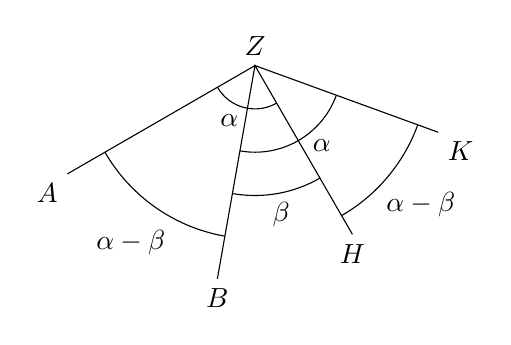
\begin{tikzpicture}[scale=.55]
\coordinate (Z) at (0,0);
\coordinate (A) at (-150:5cm);
\coordinate (B) at (-100:5cm);
\coordinate (H) at (-60:4.5cm);
\coordinate (K) at (-20:4.5cm);
\draw (A) node[below left] {$A$} -- (Z) node[above] {$Z$} -- (B) node[below] {$B$};
\draw (H) node[below] {$H$} -- (Z) -- (K) node[below right] {$K$};
\draw (-150:1cm) arc (-150:-60:1);
\draw (-100:2cm) arc (-100:-20:2);
\draw (-100:3cm) arc (-100:-60:3);
\draw (-150:4cm) arc (-150:-100:4);
\draw (-60:4cm) arc (-60:-20:4);
\node at (-115:1.4) {$\alpha$};
\node at (-50:2.4) {$\alpha$};
\node at (-80:3.5) {$\beta$};
\node at (-40:5) {$\alpha - \beta$};
\node at (-125:5) {$\alpha - \beta$};
\end{tikzpicture}
\caption{$\angle AZB=\angle HZK$}\label{f.compass-relative4}
\end{subfigure}
\end{center}
\end{figure}

%%%%%%%%%%%%%%%%%%%%%%%%%%%%%%%%%%%%%%%%%%%%%%%%%%%%%%%%%%%%%%%

\section{מציאת נקודת החיתוך של שני ישרים}
\label{s.two-lines}

\begin{theorem}
נתונים שני ישרים (שאינם מקבילים) המכילים את הקטעים
$\overline{AB},\overline{CD}$,
ניתן לבנות את
$S$,
נקודת החיתוך של הישרים.
\end{theorem}
\begin{proof}
נבנה את
$C',D'$,
השיקופים של
$C,D$
ביחס ל-%
$\overline{AB}$.
ישנם שני מקרים, תלוי אם 
$C,D$ 
נמצאות משני צדדיו של
$\overline{AB}$
או באותו צד, כפי שניתן לראות באיורים%
~\ref{f.compass-intersection1}, \ref{f.compass-intersection2}.
נסמן את קטעי הקו 
$c,d,e,x$
לפני האיורים.

\textbf{מקרה $1$:}
$C,D$ 
נמצאות בצדדים שונים של
$\overline{AB}$.
נקודת החיתוך
$S$
נמצאת על 
$\overline{AB}$
כי
$\triangle CZS\cong \triangle C'ZS$
לפי צלע, זווית, צלע:
$\overline{CZ}=\overline{C'Z}$,
$\angle CZS = \angle C'ZS = 90^\circ$
ו-%
$\overline{ZS}$
צלע משותפת. מכאן ש-%
$\overline{C'S}=\overline{CS}$
ובאופן דומה
$\overline{D'S}=\overline{DS}$.
$\triangle CSC'\sim\triangle DSD'$
ולכן
$\disfrac{x}{e-x} = \disfrac{c}{d}$.
נפתור את המשוואה עבור
$x$
ונקבל
$x=\disfrac{c}{c+d}e$.
\begin{figure}[tb]
\begin{center}
\begin{tikzpicture}[scale=.8]
\coordinate (A) at (-4,0);
\coordinate (B) at (2,0);
\coordinate (C) at (-3,2);
\coordinate (D) at (1,-1);
\coordinate (Cp) at (-3,-2);
\coordinate (Dp) at (1,1);
\vertex{A};
\vertex{B};
\node[below] at (A) {$A$};
\node[below] at (B) {$B$};
\node[above] at (C) {$C$};
\node[below] at (D) {$D$};
\node[below] at (Cp) {$C'$};
\node[above] at (Dp) {$D'$};
\draw[name path=ab] ($(A)!1.3!(B)$) -- ($(B)!1.3!(A)$);
\draw[name path=cd] ($(C)!1.2!(D)$) -- ($(D)!1.1!(C)$);
\path [name intersections={of=ab and cd,by={S}}];
\node[above] at (S) {$S$};
\draw (Cp) -- node[below] {$x$} (S);
\draw (S) -- node[above,xshift=-5pt] {$e\!-\!x$} (Dp);
\draw (C) -- node[above left,yshift=6pt] {$c$} (Cp);
\draw (D) -- node[above right,yshift=6pt] {$d$} (Dp);
\path (C) -- node[right,xshift=2pt] {$x$} (S);
\path (S) -- node[left,near end,xshift=-2pt] {$e\!-\!x$} (D);
\node[below left] at (C|-A) {$Z$};
\vertex{C};
\vertex{D};
\vertex{Cp};
\vertex{Dp};
\draw ($(C)!.5!(Cp)$) rectangle +(6pt,6pt);
\draw[rotate=90] ($(D)!.5!(Dp)$) rectangle +(6pt,6pt);
\end{tikzpicture}
\end{center}
\caption{בניית החיתוך של שני ישרים (1)}\label{f.compass-intersection1}
\end{figure}

\textbf{מקרה $2$:}
$C,D$ 
נמצאות באותו צד של
$\overline{AB}$.
$\triangle CSC'\sim\triangle DSD'$,
ולכן
$\disfrac{x}{x-e}=\disfrac{c}{d}$
ונקבל 
$x=\disfrac{c}{c-d}e$.

\begin{figure}[tb]
\begin{center}
\begin{tikzpicture}[scale=.8]
\coordinate (A) at (-4,0);
\coordinate (B) at (2,0);
\coordinate (C) at (-3,2);
\coordinate (D) at (-1,1);
\coordinate (Cp) at (-3,-2);
\coordinate (Dp) at (-1,-1);
\vertex{A};
\vertex{B};
\node[below] at (A) {$A$};
\node[below] at (B) {$B$};
\node[above] at (C) {$C$};
\node[above] at (D) {$D$};
\node[below] at (Cp) {$C'$};
\node[below] at (Dp) {$D'$};
\draw[name path=ab] ($(A)!1.3!(B)$) -- ($(B)!1.3!(A)$);
\draw[name path=cd] ($(C)!2.2!(D)$) -- ($(D)!1.1!(C)$);
\path [name intersections={of=ab and cd,by={S}}];
\node[above] at (S) {$S$};
\draw (Cp) -- (S);
\draw (C) -- node[above left,yshift=6pt] {$c$} (Cp);
\draw (D) -- node[above right,yshift=6pt] {$d$} (Dp);
\path (C) -- node[above] {$e$} (D);
\path (Cp) -- node[below] {$e$} (Dp);
\path (D) -- node[above right,xshift=-4pt] {$x-e$} (S);
\path (Dp) -- node[below right,xshift=-4pt] {$x-e$} (S);
\node[below left] at (C|-A) {$Z$};
\vertex{C};
\vertex{D};
\vertex{Cp};
\vertex{Dp};
\draw ($(C)!.5!(Cp)$) rectangle +(6pt,6pt);
\draw[rotate=90] ($(D)!.5!(Dp)$) rectangle +(6pt,6pt);
\end{tikzpicture}
\end{center}
\caption{בניית החיתוך של שני ישרים (2)}\label{f.compass-intersection2}
\end{figure}
נבנה את המעגלים
$c(C',d)$,
$c(D,e)$
ונסמן את נקודת החיתוך שלהם על הקו 
$\overline{CC'}$
ב-%
$H$
(איור%
~\ref{f.compass-intersection3}).
סכום האורכים של
$\overline{CC'},\overline{C'H}$
הוא
$c + d$.
עלינו להראות ש-%
$H$
נמצאת על המשך 
$\overline{CC'}$,
כך ש-%
$\overline{CH}$
הוא קטע באורך
$c+d$.
במקרה ש-%
$C,D$
נמצאות באותו צד של
$\overline{AB}$, 
$\overline{CH} = c - d$
(לא מופיע באיור).

\begin{figure}[tb]
\begin{center}
\begin{tikzpicture}[scale=.8]
\coordinate (A) at (-4,0);
\coordinate (B) at (2,0);
\coordinate (C) at (-3,2);
\coordinate (D) at (1,-1);
\coordinate (Cp) at (-3,-2);
\coordinate (Dp) at (1,1);
\vertex{A};
\vertex{B};
\node[below left] at (A) {$A$};
\node[below] at (B) {$B$};
\node[above] at (C) {$C$};
\node[below] at (D) {$D$};
\node[left] at (Cp) {$C'$};
\node[above] at (Dp) {$D'$};
\draw[name path=ab] ($(A)!1.3!(B)$) -- ($(B)!1.3!(A)$);
\draw[name path=cd] ($(C)!1.2!(D)$) -- ($(D)!1.1!(C)$);
\path [name intersections={of=ab and cd,by={S}}];
\node[above,yshift=4pt] at (S) {$S$};
\draw (Cp) -- node[below right,xshift=5pt,yshift=5pt] {$e$} (Dp);
\path (C) -- node[above left] {$c$} (Cp);
\draw[thick,dashed] (D) -- node[above right] {$d$} (Dp);
\draw[name path=circled] (D) let
  \p1 = ($ (D) - (C) $),
  \n2 = {veclen(\x1,\y1)}
in
  ++(130:\n2) arc (130:230:\n2);

\draw[name path=circlecp] (Cp) let
  \p1 = ($ (D) - (Dp) $),
  \n2 = {veclen(\x1,\y1)}
in
  ++(-180:\n2) arc (-180:0:\n2);
\path [name intersections={of=circled and circlecp,by={H}}];
\node[below left] at (H) {$H$};
\draw ($(C)!1.2!(H)$) -- (C);
\draw (H) -- node[right] {$d$} (Cp);
\draw (D) -- node[right,xshift=18pt,yshift=12pt] {$e$} (H);
\vertex{Cp};
\vertex{D};
\vertex{C};
\vertex{Dp};
\vertex{H};
\path (C) -- node[above] {$x$} (S);
\path (Cp) -- node[below] {$x$} (S);
\end{tikzpicture}
\end{center}
\caption{בניית החיתוך של שני ישרים (3)}\label{f.compass-intersection3}
\end{figure}


$H$
היא החיתוך של 
$c(C',d),c(D,e)$,
ולכן
$\overline{C'H}=d,\overline{DH}=e$.
לפי הבנייה 
$\overline{C'D'}=e, \overline{DD'}=d$,
ולכן המרובע
$C'D'DH$
הוא מקבילית. 
\begin{figure}[tb]
\begin{center}
\begin{tikzpicture}[scale=.9]
\coordinate (A) at (-4,0);
\coordinate (B) at (2,0);
\coordinate (C) at (-3,2);
\coordinate (D) at (1,-1);
\coordinate (Cp) at (-3,-2);
\coordinate (Dp) at (1,1);
\vertex{A};
\vertex{B};
\node[below left] at (A) {$A$};
\node[below] at (B) {$B$};
\node[above] at (C) {$C$};
\node[below] at (D) {$D$};
\node[left] at (Cp) {$C'$};
\node[above] at (Dp) {$D'$};
\draw[name path=ab] ($(A)!1.3!(B)$) -- ($(B)!1.3!(A)$);
\draw[name path=cd] ($(C)!1.2!(D)$) -- ($(D)!1.1!(C)$);
\path [name intersections={of=ab and cd,by={S}}];
\node[above,yshift=4pt] at (S) {$S$};
\draw (Cp) -- (Dp);
\path (C) -- node[above,yshift=4pt] {$x$} (S);
\path (Cp) -- node[below,yshift=-4pt] {$x$} (S);
\path (C) -- node[above left] {$c$} (Cp);
\draw (D) -- node[above right] {$d$} (Dp);
\draw[name path=circled] (C) let
  \p1 = ($ (S) - (C) $),
  \n2 = {veclen(\x1,\y1)}
in
  ++(-10:\n2) arc (-10:-100:\n2);

\draw[name path=circlecp] (Cp) let
  \p1 = ($ (S) - (C) $),
  \n2 = {veclen(\x1,\y1)}
in
  ++(100:\n2) arc (100:0:\n2);
\draw (Cp) -- (C);
\vertex{C};
\vertex{Cp};
\vertex{D};
\vertex{Dp};
\end{tikzpicture}
\end{center}
\caption{בניית החיתוך של שני ישרים (4)}\label{f.compass-intersection4}
\end{figure}

לפי הבנייה
$\overline{DD'}\|\overline{CC'}$,
ולכן
$\overline{C'H}\|\overline{DD'}$
וגם
$\overline{C'H}\|\overline{CC'}$.
מכיוון שאחת מנקודות הקצה של הקטע היא
$C'$ת
היא חייבת להיות על הישר המכיל את
$\overline{CC'}$.
לפי משפט%
~\ref{thm.add-subtract-mm},
מהאורכים הנתונים
$c,d,e$
ניתן לבנות קטע באורך
$c+d$,
ולפי משפט
\ref{thm.ratio}
ניתן לבנות קטע באורך
$x=\disfrac{c}{c+d}e$.
$S$,
נקודת החיתוך של המעגלים
$c(C,x)$
ו-%
$c(C',x)$,
היא גם נקודת החיתוך של
$\overline{AB}, \overline{CD}$
(איור%
~\ref{f.compass-intersection4}).
\end{proof}

%%%%%%%%%%%%%%%%%%%%%%%%%%%%%%%%%%%%%%%%%%%%%%%%%%%%%%%%%%%%%%%

\section{מציאת נקודת החיתוך של ישר ומעגל}\label{s.line-circle}

\begin{theorem}
נתונים מעגל
$k=C(M,r)$
וישר
$l$,
ניתן לבנות את 
$X,Y$,
נקודות החיתוך של 
$k,l$.
\end{theorem}
\begin{proof}
נבנה את
$M'$,
השיקוף של
$M$
ביחס ל-%
$l$,
ואת המעגל
$k'=c(M',r)$.
$MYM'\cong\triangle MXM'$, 
ולכן 
$X,Y$,
הן נקודות החיתוך של
$l$
ו-%
$k$
(איור%
~\ref{f.compass-circle4}).

\begin{figure}[t]
\begin{center}
\begin{tikzpicture}[scale=.5]
\coordinate (A) at (-7,0);
\coordinate (B) at (8,0);
\coordinate (M) at (0,-2);
\coordinate (Mp) at (0,2);
\node[below left] at (M) {$M$};
\node[above left] at (Mp) {$M'$};
\draw[name path=c1] (M) circle[radius=3cm];
\draw[name path=c2] (Mp) circle[radius=3cm];
\draw[name path=ab] ($(A)!1.2!(B)$) --
  node[above,very near end] {$l$} ($(B)!1.2!(A)$);
\path [name intersections={of=c1 and c2,by={S1,S2}}];
\path[name path=radius1] (M) -- ++(15:4cm);
\path [name intersections={of=c1 and radius1,by={R1}}];
\draw (M) -- node[below] {$r$} (R1);
\path[name path=radius2] (Mp) -- ++(40:4cm);
\path [name intersections={of=c2 and radius2,by={R2}}];
\draw (Mp) -- node[above] {$r$} (R2);
\draw (Mp) -- (M) -- (S1) -- (Mp) -- (S2) -- (M);
\node[right,xshift=6pt,yshift=6pt] at (S1) {$X$};
\node[left,xshift=-6pt,yshift=6pt] at (S2) {$Y$};
\draw (0,0) rectangle +(10pt,10pt);
\node at (-3.5,-3) {$k$};
\node at (-3.5,3) {$k'$};
\end{tikzpicture}
\end{center}
\caption{בניית החיתוך של ישר ומעגל (1)}\label{f.compass-circle4}
\end{figure}

בנייה זו אינה אפשרית אם מרכז המעגל
$M$
נמצא על הקו
$l$.
במקרה זה, נבחר נקודה שרירותית 
$A$
על
$l$
שמרחקה
 מ-%
$M$
גדול מ-%
$r$.
לפי משפט~%
~\ref{thm.add-subtract-mm}
נאריך או נקצר את
$\overline{AM}$
ב-%
$r$.
$X,Y$
נקודות הקצה של קטעים אלו, הן נקודות החיתוך של
$k$
ו-%
$l$
(איור%
~\ref{f.compass-circle5}).
\end{proof}
\begin{figure}[b]
\begin{center}
\begin{tikzpicture}[scale=.5]
\coordinate (A) at (-7,0);
\coordinate (B) at (8,0);
\coordinate (M) at (0,0);
\vertex{M};
\vertex{A};
\node[below] at (A) {$A$};
\node[below left] at (M) {$M$};
\draw[name path=c1] (M) circle[radius=3cm];
\draw[name path=ab] ($(A)!1.2!(B)$) -- 
  node[above,very near end] {$l$} ($(B)!1.2!(A)$);
\path[name path=radius1] (M) -- ++(50:4cm);
\path [name intersections={of=c1 and radius1,by={R1}}];
\draw (M) -- node[above] {$r$} (R1);
\path [name intersections={of=c1 and ab,by={S1,S2}}];
\node[above right] at (S1) {$X$};
\node[above left] at (S2) {$Y$};
\path (M) -- node[below,xshift=4pt] {$\overline{AM}+r$} (S1);
\path (A) -- node[below] {$\overline{AM}-r$} (S2);
\node at (-2.5,2.5) {$k$};
\end{tikzpicture}
\end{center}
\caption{בניית החיתוך של קו מעגל (2)}\label{f.compass-circle5}
\end{figure}

%%%%%%%%%%%%%%%%%%%%%%%%%%%%%%%%%%%%%%%%%%%%%%%%%%%%%%%%%%%%%%%

\newpage

\subsection*{מהי ההפתעה?}

כאשר לומדים על בנייה בסרגל ובמחוגה, ברור מאליו ששני הכלים נחוצים, ולכן מפתיע מאוד לגלות שמחוגה בלבד מספיקה. ההוכחה די ארוכה כך שלא נשאיר את הסרגל בבית, אבל המשפט מראה שאין להניח שאין חלופות למושגים מתמטיים ידועים.

%%%%%%%%%%%%%%%%%%%%%%%%%%%%%%%%%%%%%%%%%%%%%%%%%%%%%%%%%%%%%%%

\subsection*{מקודות}

פרק זה מבוסס על בעיה מספר 33
ב-%
\cite{dorrie1}
ועל העיבוד שלה על ידי מיכאל וולטרמן
\L{(Michael Woltermann)} 
\cite{dorrie2}.
הוכחה נוספת ניתן למצוא ב-%
\cite{mm}.
